\documentclass{article}
\usepackage{verbatim}
\usepackage{amsmath}
\usepackage{amssymb}
\usepackage{hyperref}
\usepackage{graphicx}
\usepackage{color}
\newcommand{\red}[1]{{\color{red}{#1}}}
\newcommand{\blue}[1]{{\color{blue}{#1}}}

\usepackage{xy}
\xyoption{all}

\usepackage[a4paper,
            bindingoffset=0.2in,
            left=1.0in,
            right=1.0in,
            top=1.0in,
            bottom=1.0in,
            footskip=.25in]{geometry}

\title{Documentation}
\author{Caleb Kennedy Hill}
\date{Summer 2026}

\begin{document}

\maketitle


\red{TODO:
    \begin{itemize}
        \item Start pipeline docs
        \item Start metrics metadata
        \item Expand ArcGIS Portfolio docs
    \end{itemize}
}

This document is intended to serve as a reference for those of us working on the UNH 
Sustainability Institute's Split Incentive Tak Force.


\section{Data Pipeline}\label{sec:pipeline}

This section will serve as documentation for the data pipeline.
The required python libraries include \verb|pandas|, \verb|us|, and \verb|census|.
There are some others that are standard.


\subsection{Setup}
The preamble/defining involves setting the dictionaries \verb|target_states|,
\verb|nems_munis|, and \verb|years|.
The \verb|us.states| module takes care of the FIPS numbers for each state.
Target municipalities (i.e., NEMS members) are taken from a master list;
formatting them correctly is a great use for a chatbot.
This output needs to be verified, though.
The years of interest will depend on the application;
however, one should not compare overlapping ACS5 datasets!
\href{
    https://www.census.gov/newsroom/blogs/random-samplings/2022/03/period-estimates-american-community-survey.html
}{Click here to see why.}


\subsection{Getting ACS5 Data}
Currently there are two different types of API calls taking place: one for housing age-related data,
and one for the rest.
This will change.

\subsubsection*{Query helpers}
Below are some useful facts about the functions used to interact with the ACS5 API.

\begin{verbatim}
    acs_df_from_raw(
        all_raw_data, 
        rename_dict:dict)
\end{verbatim}
Returns a Pandas DataFrame from raw data dumped out of the ACS5 module of the census package: 
\verb|census.acs5.state_county_subdivision|.



\begin{verbatim}
    query_states_years_variables(
        target_states:dict, 
        target_years:list, 
        variables:dict, 
        loud=True)
\end{verbatim}
Essentially a wrapper for \verb|census.acs5.state_county_subdivision|.
It manually deals with some issues with a few of the municipalities.
Some naming conventions aren't matching, so I've manually changed them.
This happens despite GEOID being a unique identifier;
it may point to a misaligned set of underlying shapefiles.
This requires further investigation.


\subsubsection*{Housing Age}
Several different functions exist which are intended to pull different ``classes'' of ACS5 variables.
For instance, \textit{Renter Landscape} (renter share, rent burder), \textit{Housing} (housing age, size),
or \textit{Energy} (energy burden, heating fuel).
The only real difference currently is between variables related to housing age and those not related
to housing age.








\subsection{Getting GIS Data}



%%%%%%%%%%%%%%%%%%%%%%%%%%%%%%%%%%%%%%%%%%%%%%%
%%%%%%%%%%%%%%%%%%%%%%%%%%%%%%%%%%%%%%%%%%%%%%%
%%%%%%%%%%%%%%%%%%%%%%%%%%%%%%%%%%%%%%%%%%%%%%%
%%%%%%%%%%%%%%%%%%%%%%%%%%%%%%%%%%%%%%%%%%%%%%%











\pagebreak

\section{ArcGIS Online}
ArcGIS Online (AGOL) is the platform on which we aggregate, filter, arrange, and ultimately deliver
information to the NEMS Network.
The basic file type for creating a map is the \textbf{shapefile}, which have suffix \verb|.shp|.
\href{https://www.youtube.com/watch?v=PfbjoAcQp8I&t=20s}{This video} gives a good enough introduction
to what a shapefile is.
The goal of the present section is to detail the process of turning \verb|.shp| files derived from \verb|GeoDataFrame|
into ArcGIS Instant Apps, for use in Portfolio projects.
The minimal system schematic is as follows:
\[
\text{Portfolio} \longleftarrow 
\text{Instant App} \longleftarrow 
\text{Web Map} \longleftarrow 
\text{Feature Layer} 
\]

For purposes, a \textbf{Portfolio} is a collection of Instant Apps, and a mini-browser to view them in.
We will be tying into the efforts of and extending the work of BU's CELT program.
With this in mind, our propotypical example of a Portfolio should be their Legacy Transition Atlas,
which is linked 
\href{https://bucas.maps.arcgis.com/apps/instant/portfolio/index.html?appid=ea07ae399445465e9dd2448f211affc0}{here.}

The AGOL platform is quite modular.
Once it is created, an Instant Apps can be specified just by URL.
This means that any products we deliver can be displayed anywhere else.
That is to say, we may have our own NEMS Portfolio existing in parellel to the CELT Portfolio.
It might be something like:
\[
\xymatrix{
    \text{NEMS Atlas} & & &  \\
    & \text{Instant App} \ar[ul] \ar[dl] & \text{Web Map} \ar[l] & \text{Feature Layer} \ar[l] \\
    \text{CELT Atlas} & & &  \\
}
\]
Once we get around to actually creating a Portfolio, we will see that the diagrams 
might be more complex.
For now, the simple one-line diagram should be a sufficient mental model.



\subsection*{Create an Instant App}
Here is where we will create the Instant Apps which will be linked inside the Portfolio.

\blue{{\bf IMPORTANT:}
To do any of this you will need an AGOL account with publishing permissions.
UNH has an AGOL license, but we need to contact admin to get permissions.
}

\begin{enumerate}

    \item 
    Prepare ShapeFiles.
    Be sure that the relevant \verb|GeoDataFrame| has been exported and compressed into a \verb|.zip| file.
    The process of obtaining the shapefiles is outlined in Section~\ref{sec:pipeline}.


    \item
    Upload the \verb|.zip| file to AGOL as a \textbf{Feature Layer}.
    Navigate to the \verb|Content| tab of AGOL, then click \verb|New item|.
    Click the \verb|Feature layer|, and then the \verb|Upload a file| otpions.
    Be sure to choose the upload option that creates a Hosted Feature Layer. \footnote{
        This step is not possible wihtout publishing permissions!
    }
    Pick a good name, and add a helpful description.

    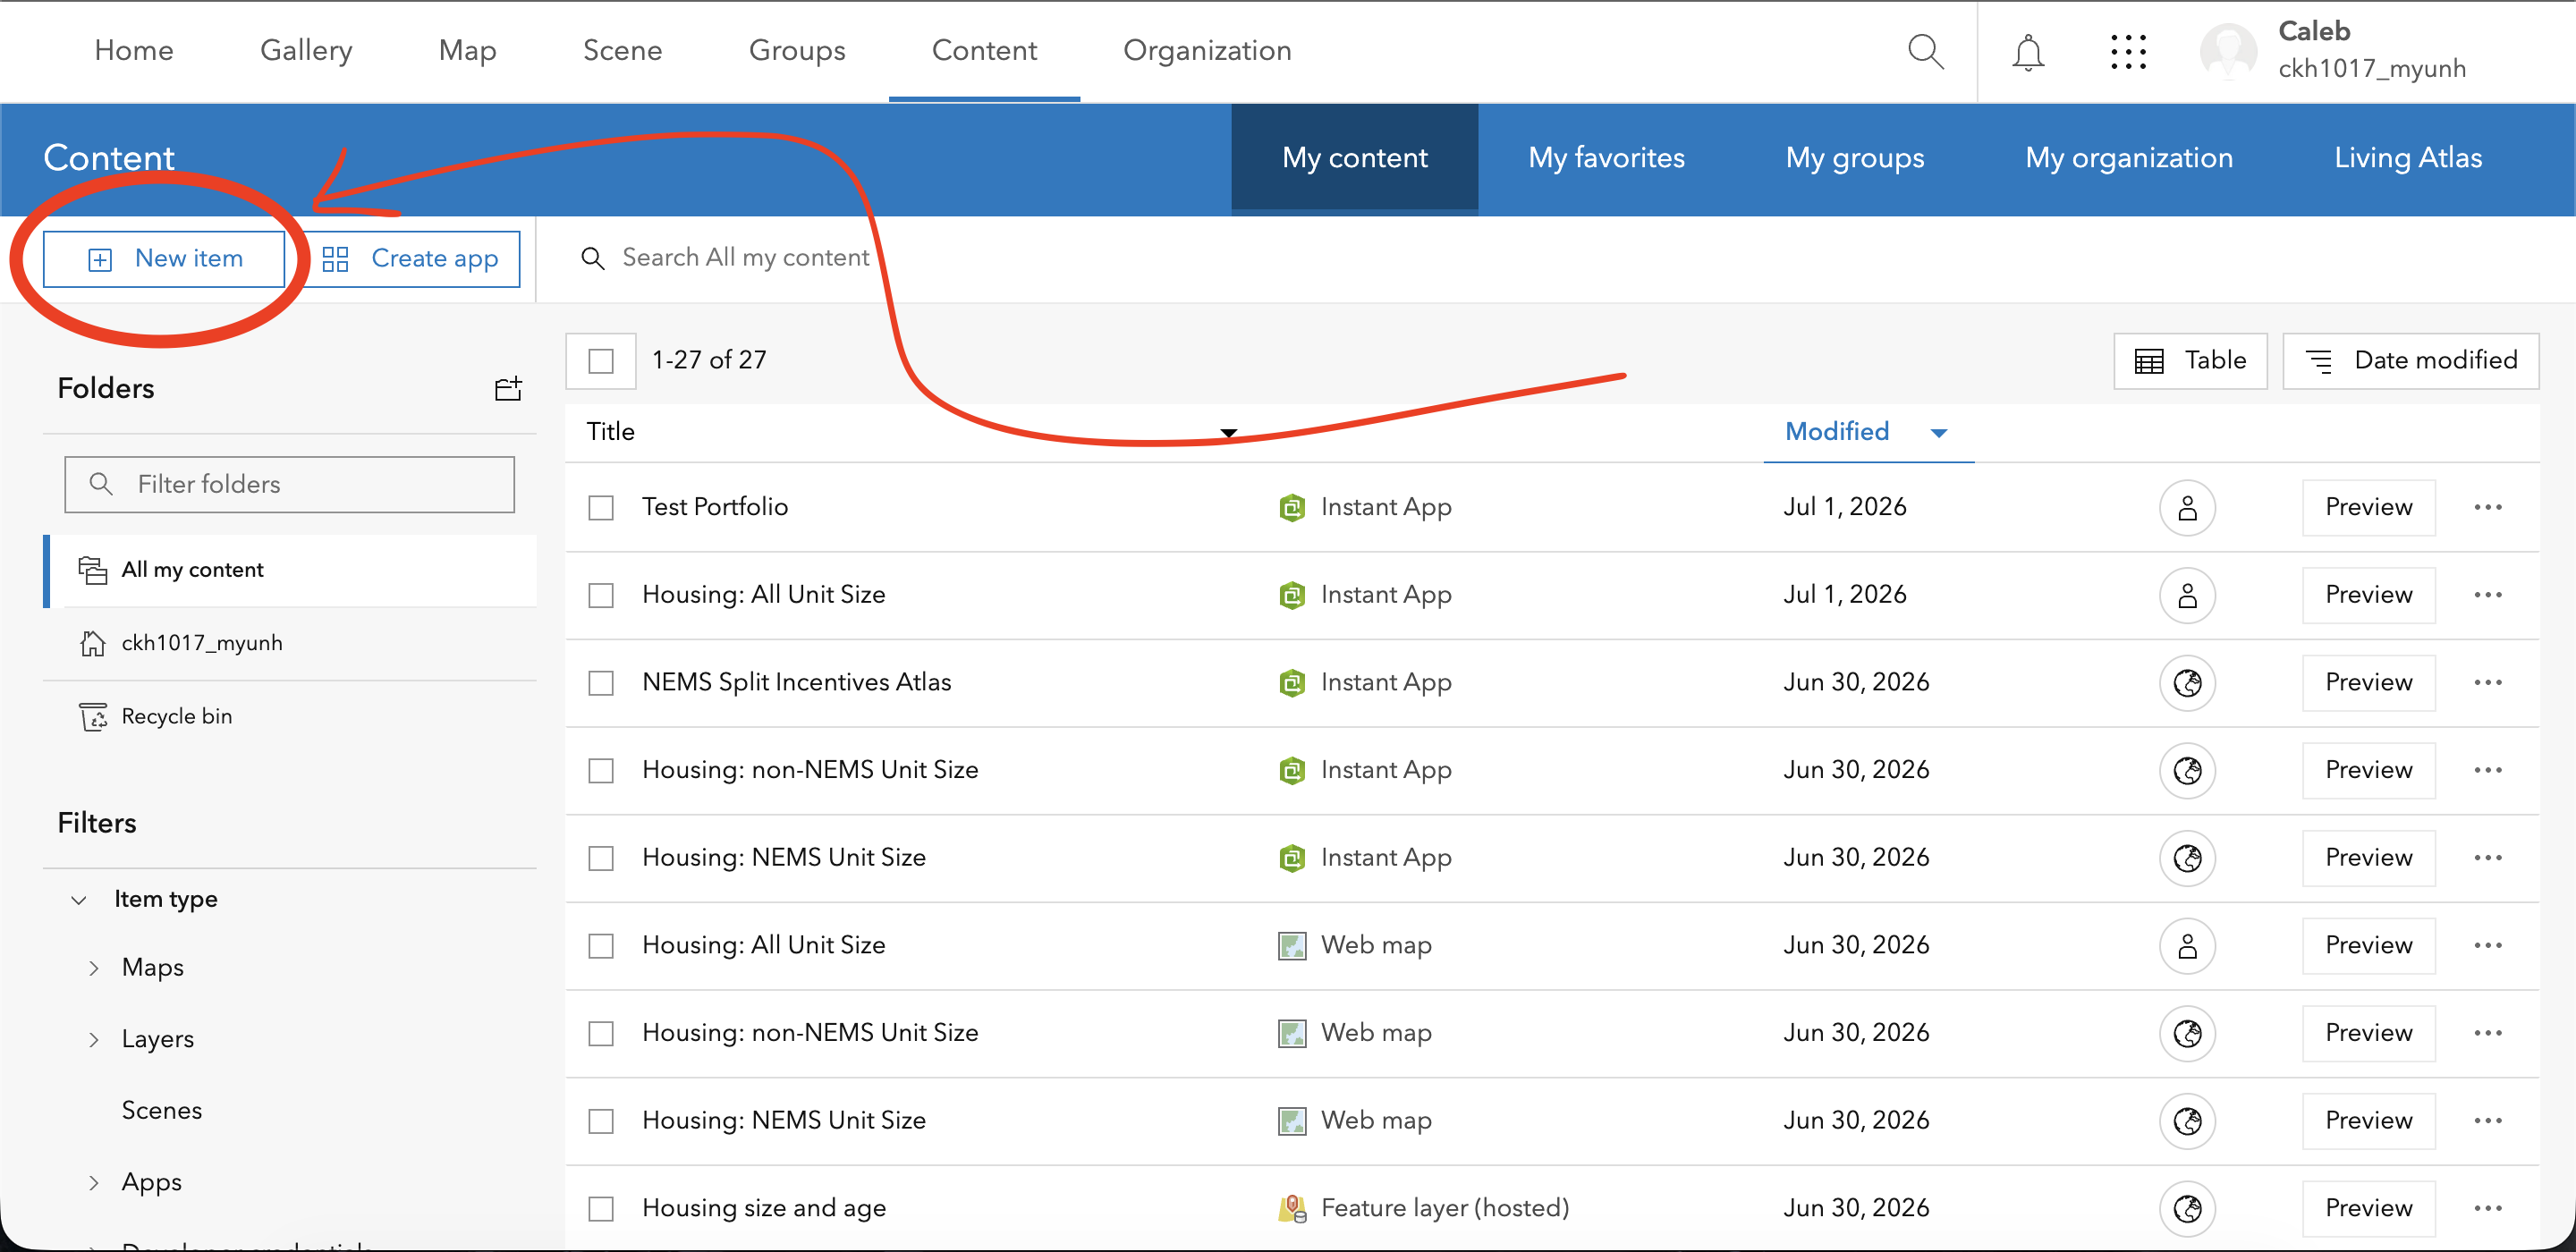
\includegraphics[width=0.75\linewidth]{screenshot_1.png}

    \item 
    Back in the \verb|Content| window, open the Hosted Feature Layer you just created.
    Choose the option to \verb|Open in Map Viewer| in the upper right.

    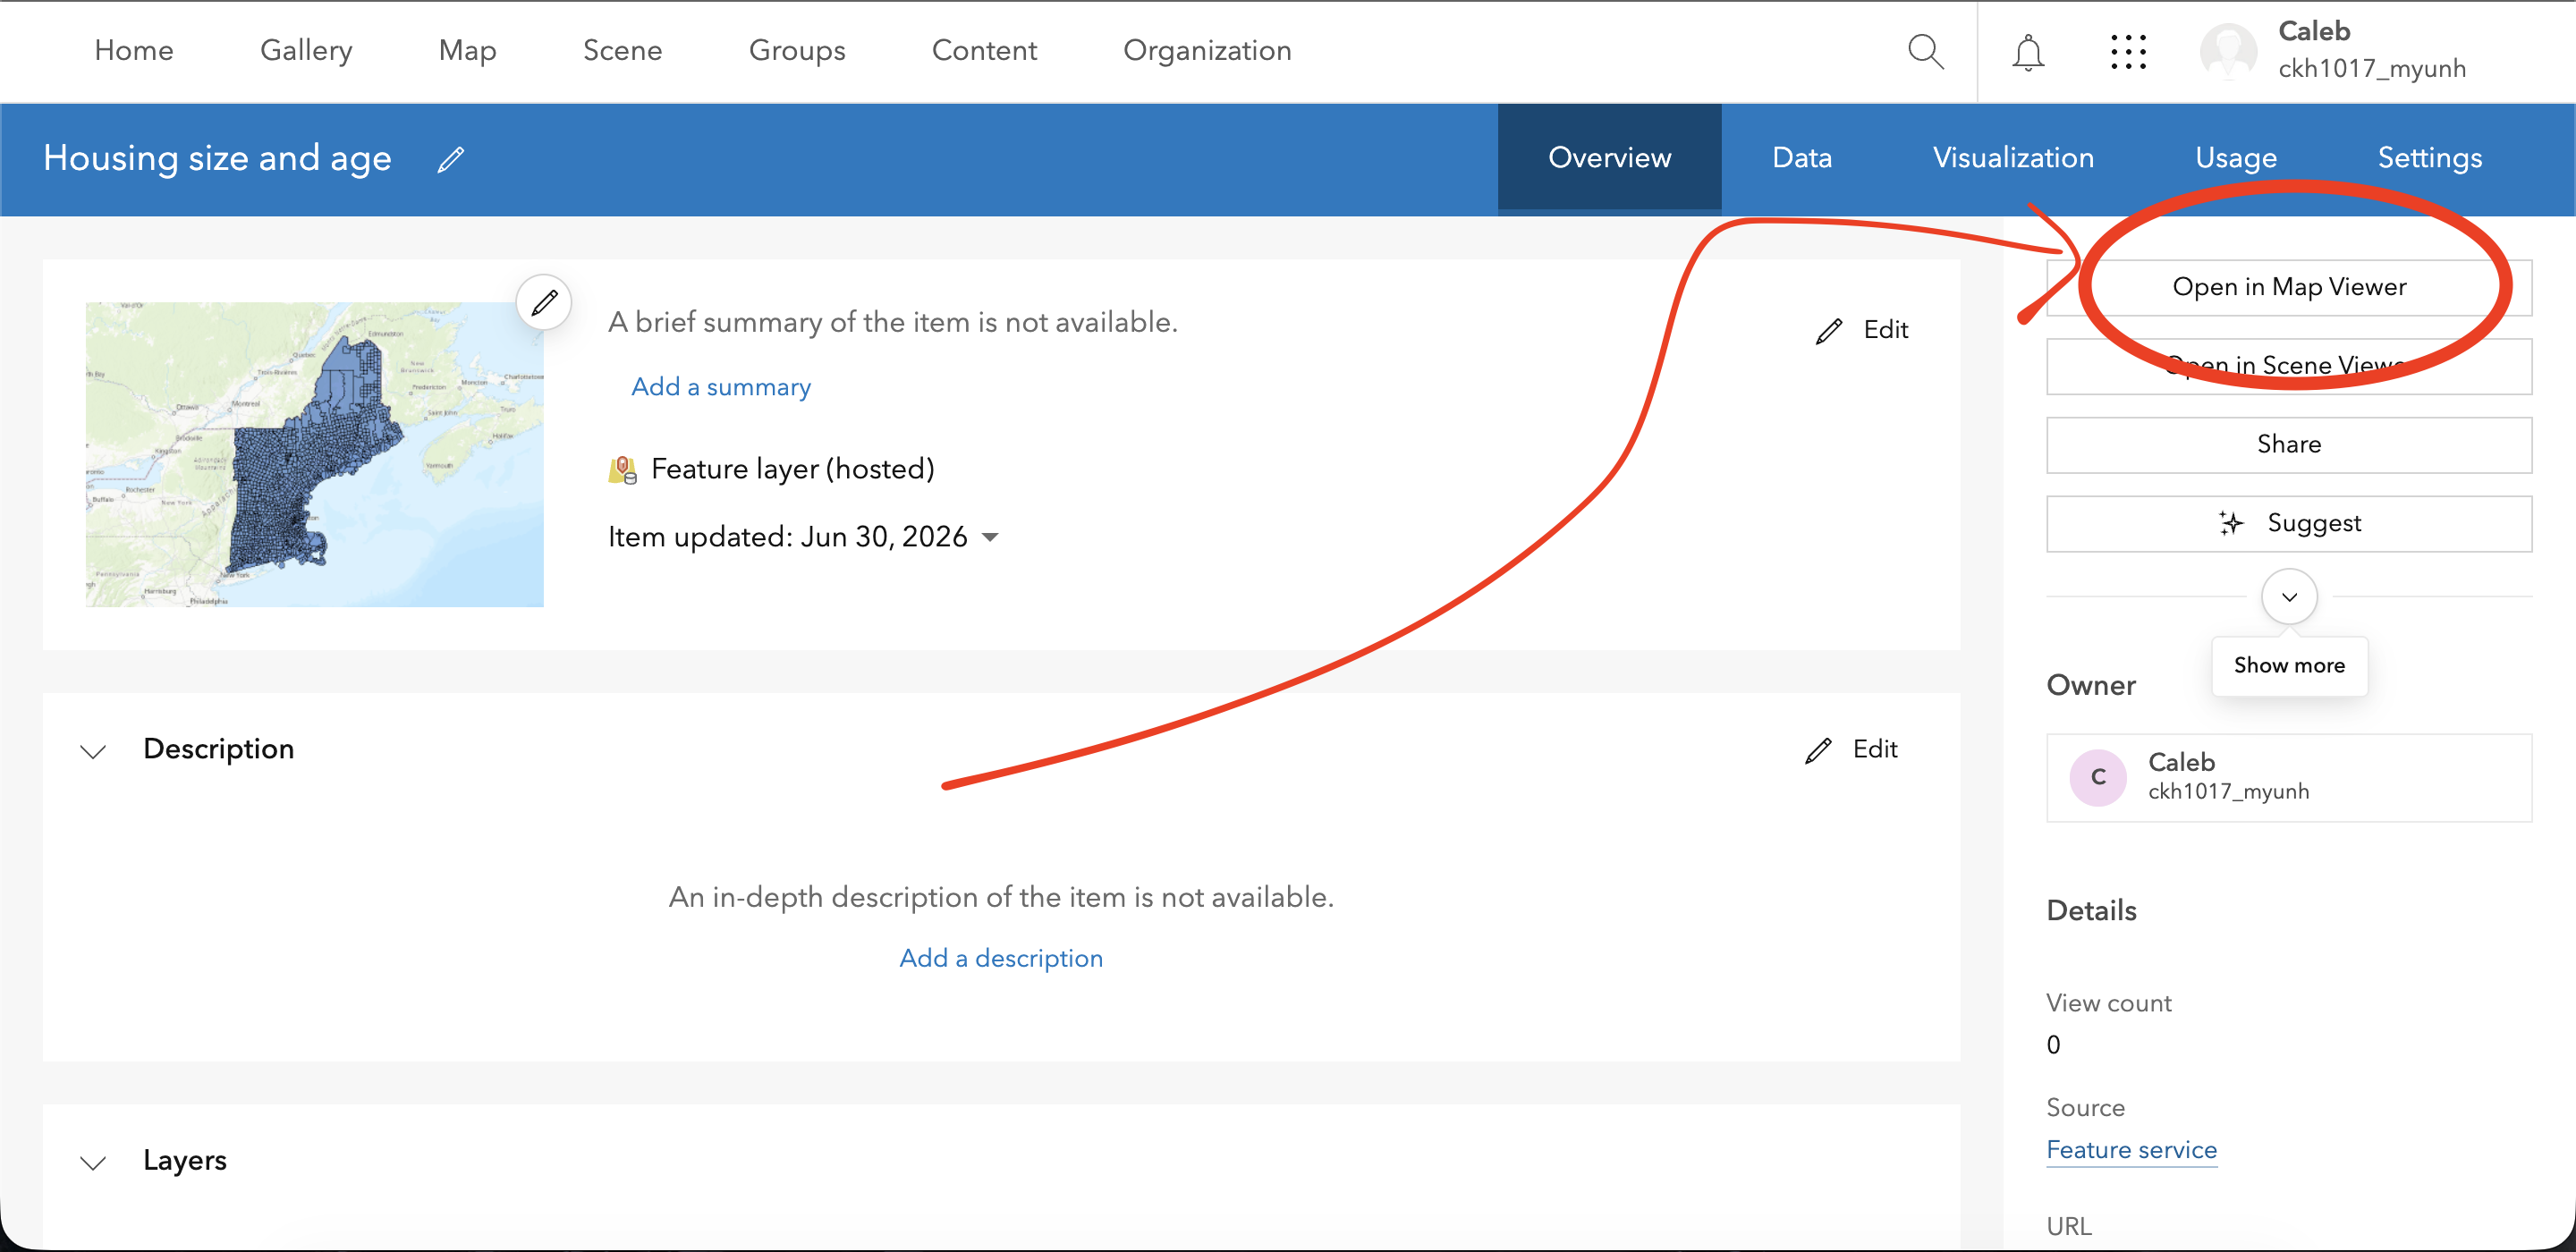
\includegraphics[width=0.75\linewidth]{screenshot_2.png}

    \item 
    Fiddle and Save.
    The righthand side of the screen has a menu for changing how the map looks. 
    We will almost exclusively tweak the top three options: Properties, Style, and Filters.
    Here are some style notes which may be standardized:
    \begin{itemize}
        \item $0\%$ transparency
        \item Continuous variables classed into three quantiles
        \item NEMS members are colored Purple 1, and non-NEMS are colored Green 5.
        If colors need to be copied exactly, they can be obtained by opening another
        map and inspecting the style options. 
    \end{itemize}

    Now is when the NEMS/non-NEMS filter shoudl be applied, i.e., filter for \verb|nems=1| or \verb|nems=0|.

    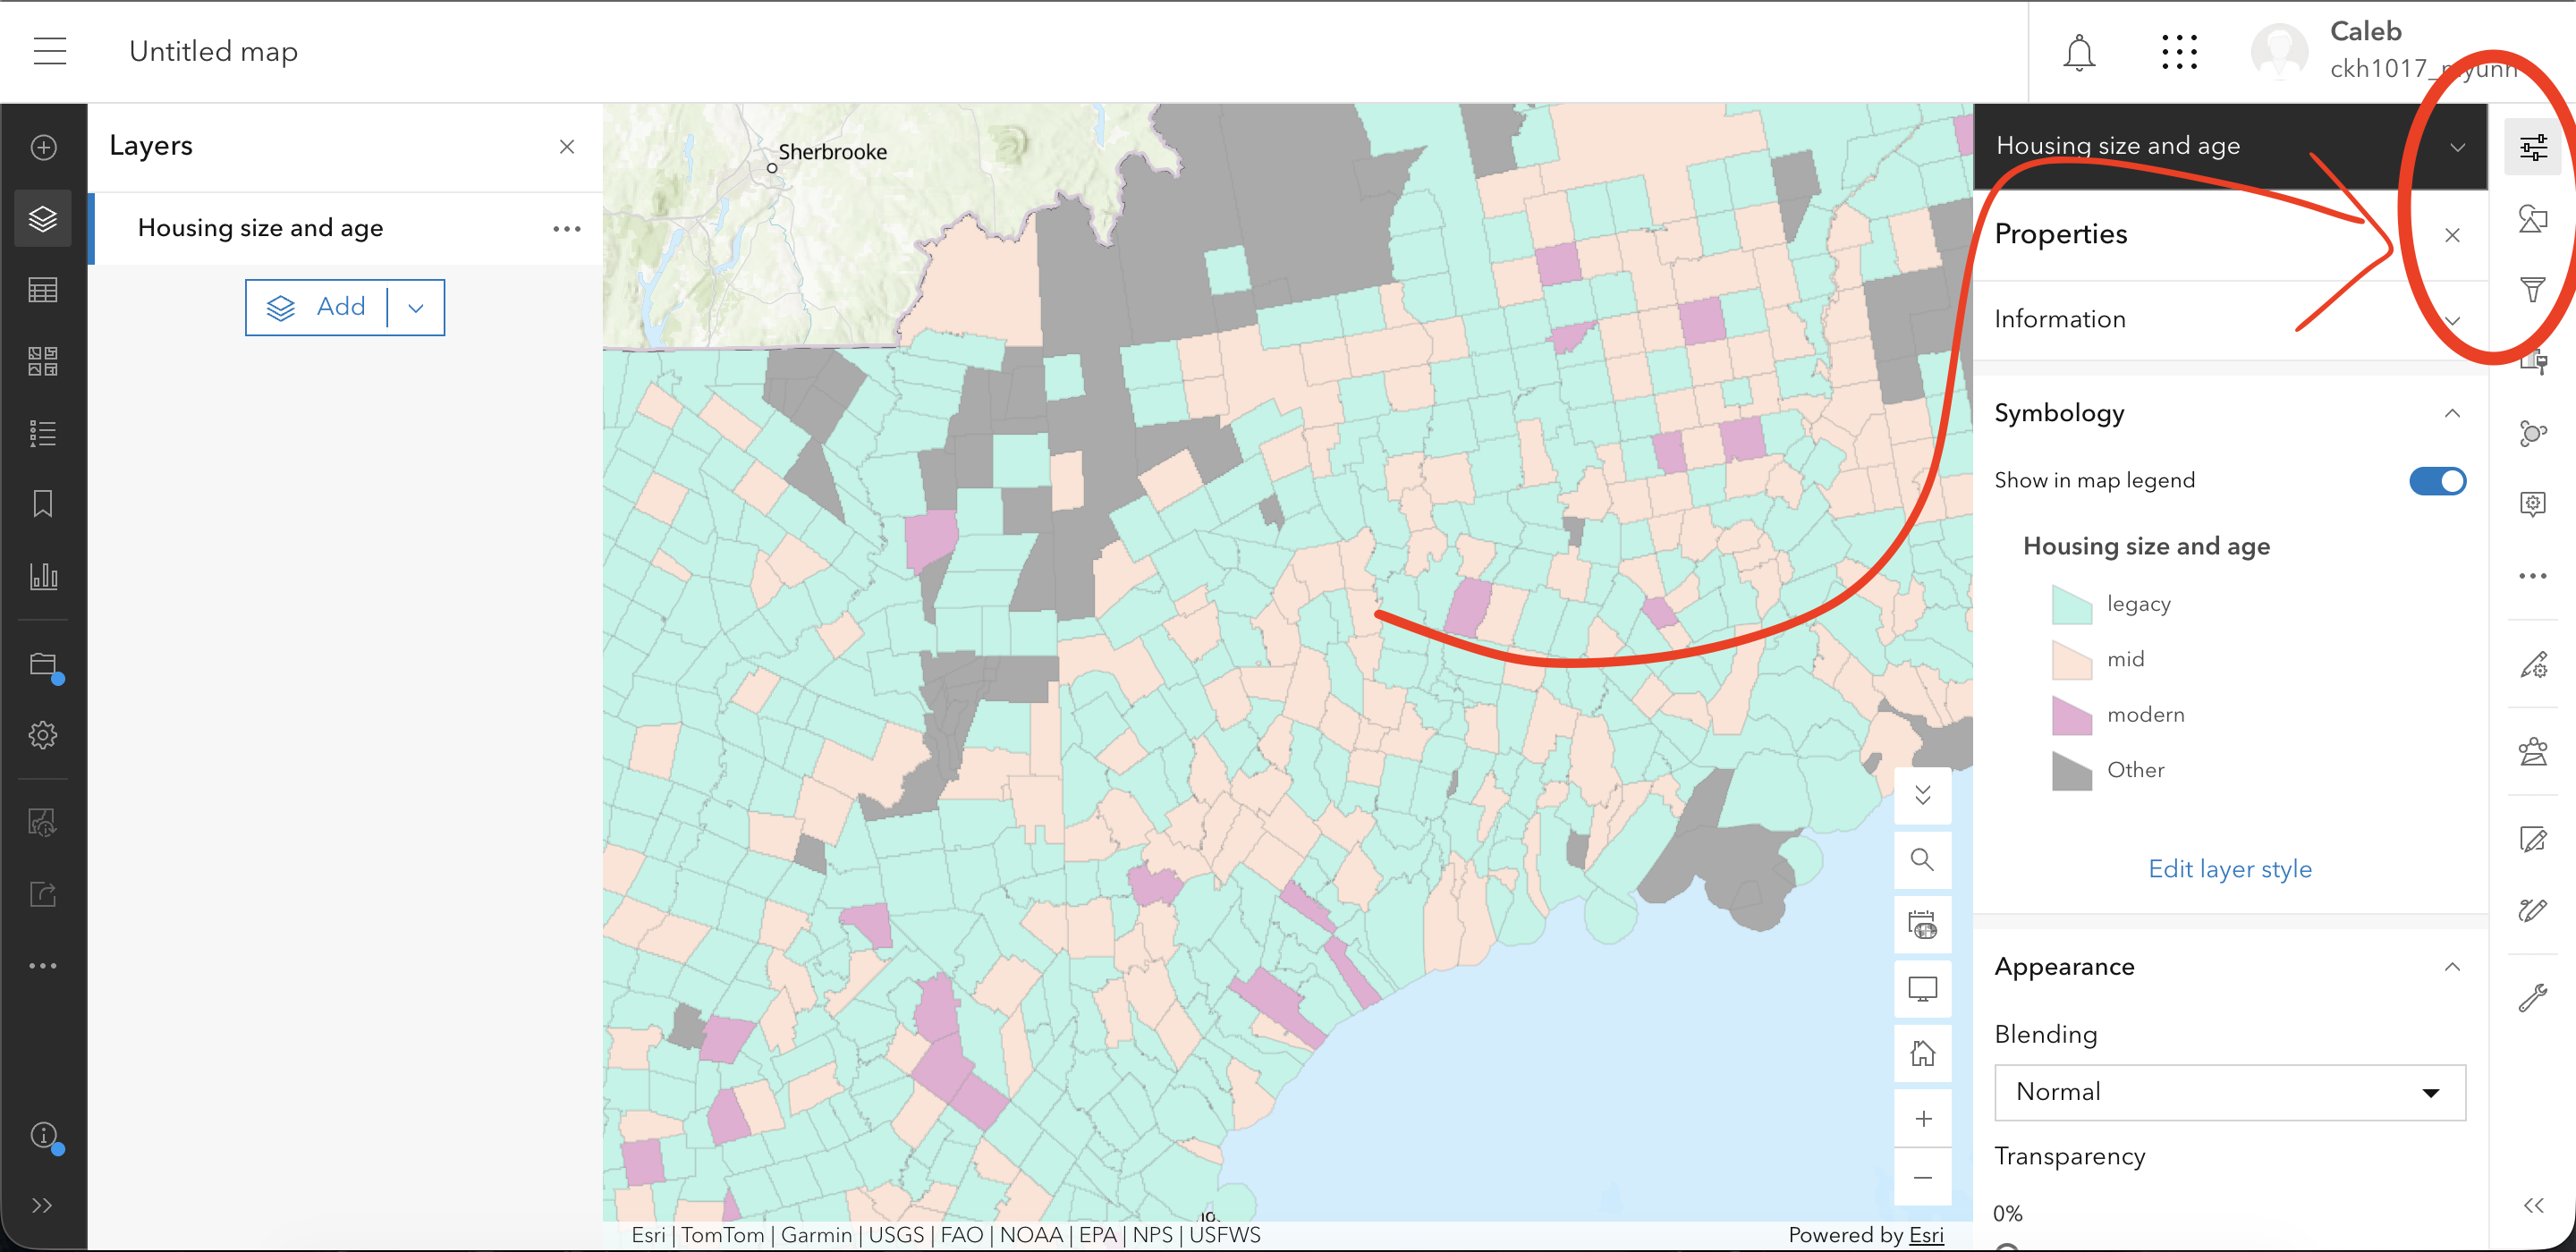
\includegraphics[width=0.75\linewidth]{screenshot_3.png}

    When you're done, click \verb|Save as| from the lefthand menu and pick the same name
    you used for the Feature Layer; add a short description as well.


    \item 
    In the \verb|Content| window, open Web Map you just created.
    In the options on the right, click \verb|Create app| and choose \verb|Instant App|.
    In the page that opens, choose the \verb|Basic (Media Map)| option.
    Name it the same thing as the previous two.
    Not much needs to change here.

    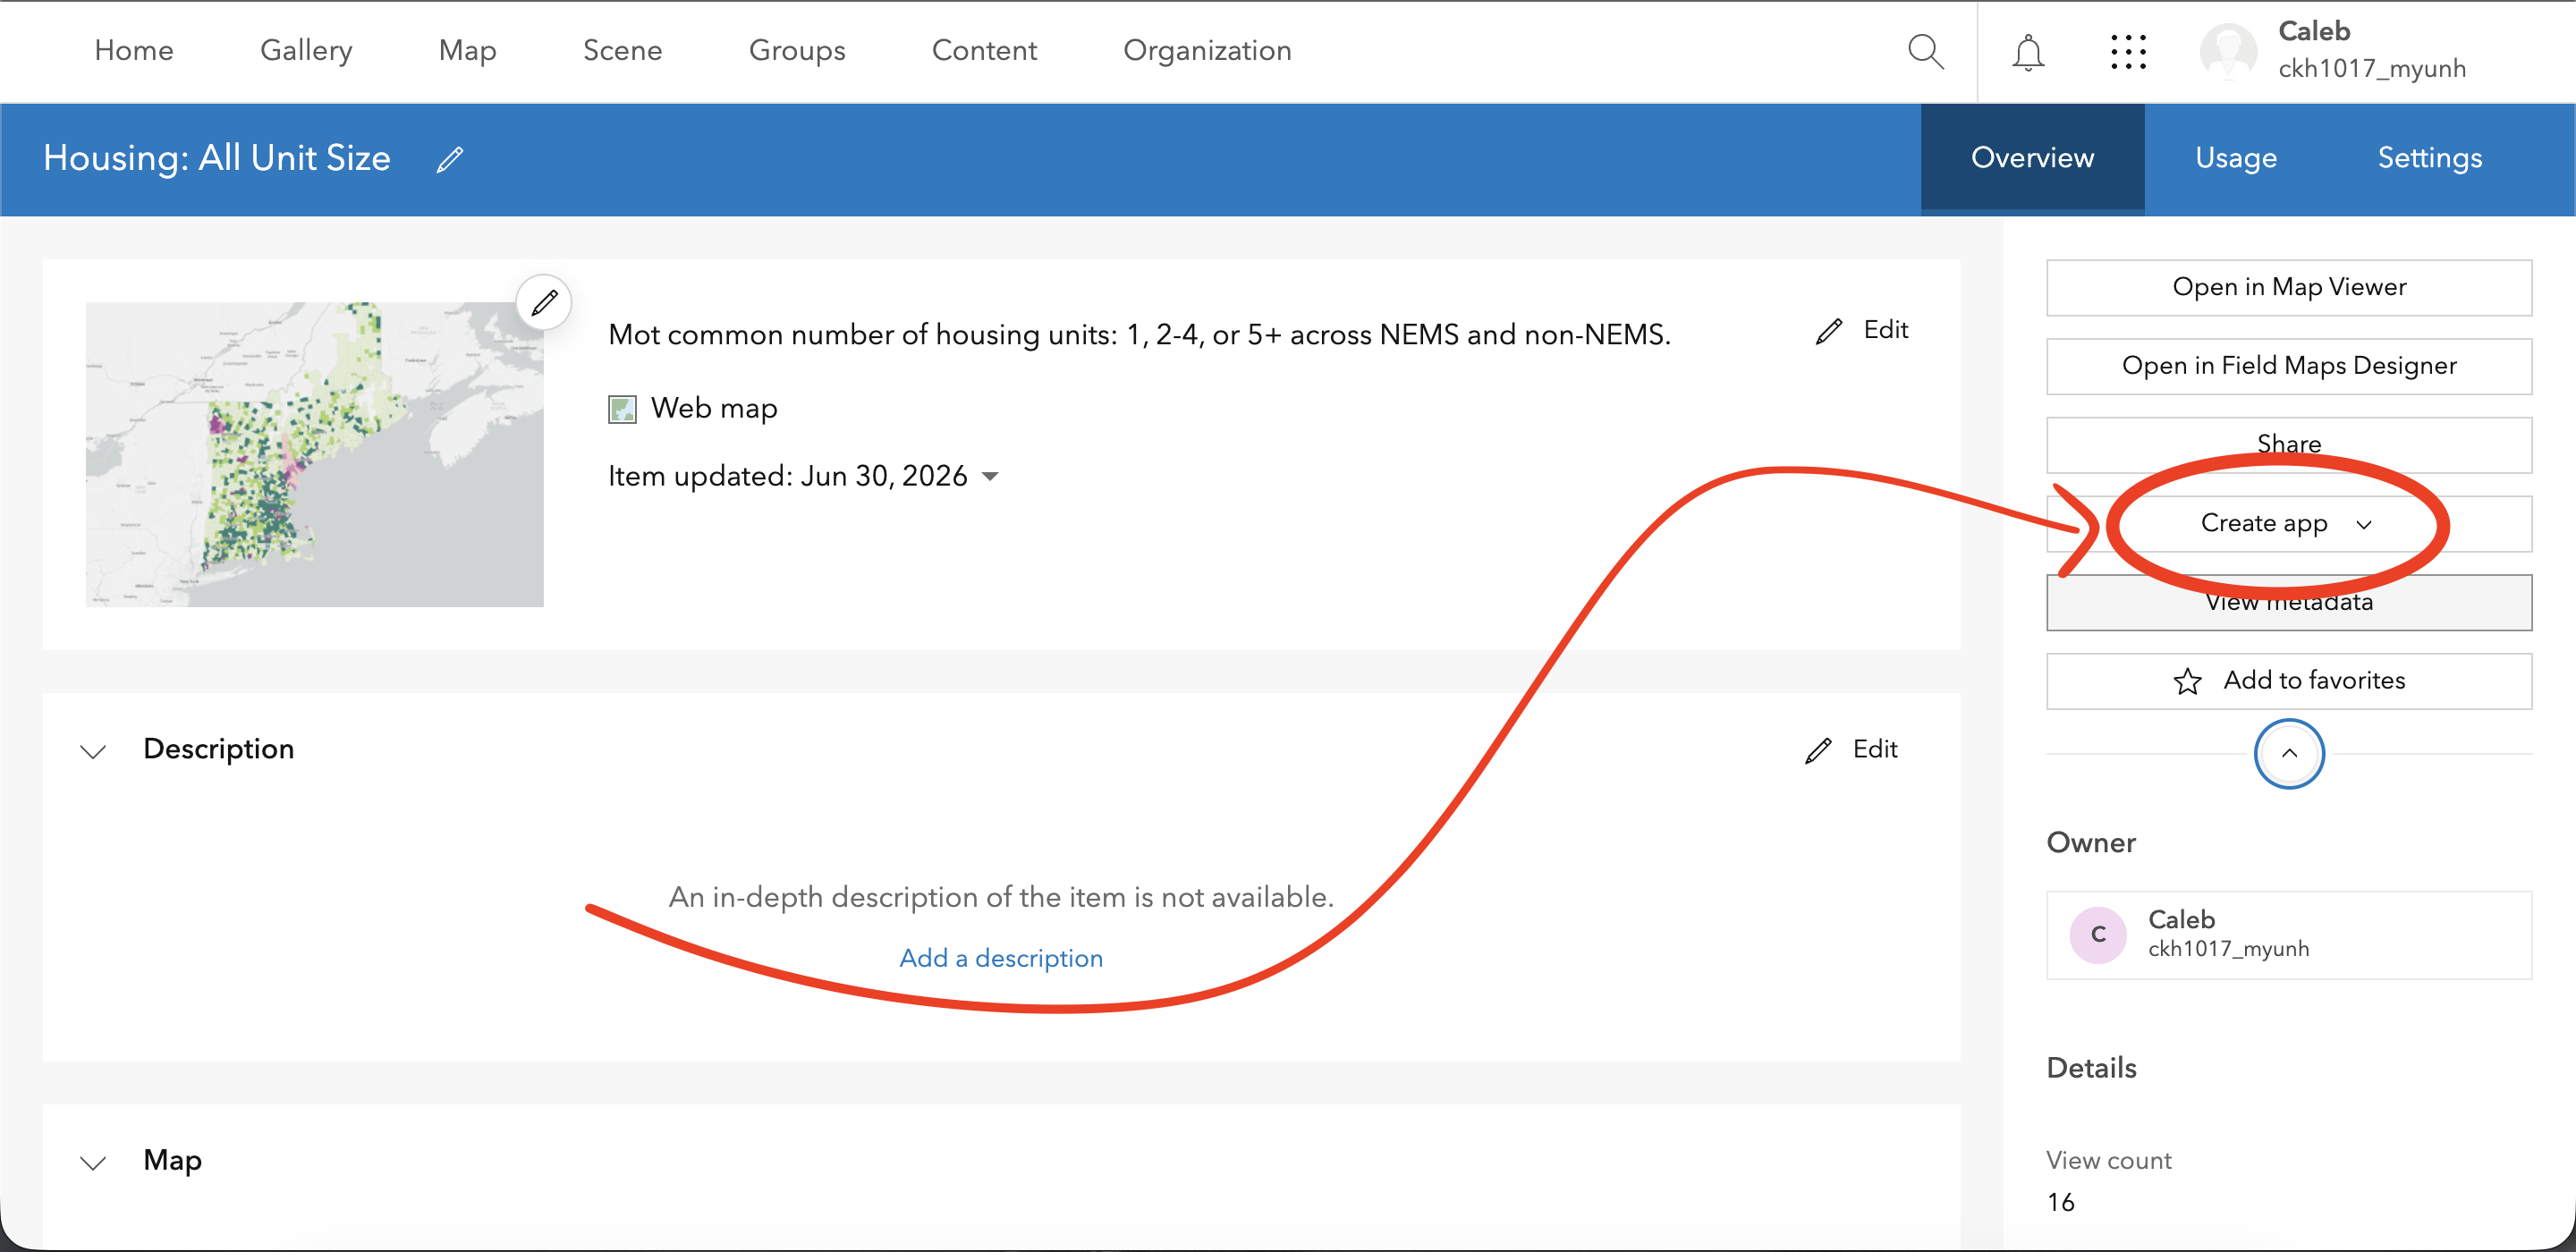
\includegraphics[width=0.75\linewidth]{screenshot_4.png}

\end{enumerate}

Thus you have created an Instant App!
This app can be shared directly via its URL.
Its default visibility is set to Private, meaning only the owner can view it.
This can be changed at the current step, or later when publishing a Portfolio.



\subsection*{Create a Portfolio}
A portfolio can house several different Instant Apps:

\[
\xymatrix@C=40pt{
    \text{Portfolio} & \text{App 1} \ar[l] & \text{Web Map 1} \ar[l] & \text{Feature Layer 1} \ar[l]\ar[dl] \\
    & \text{App 2} \ar[ul] & \text{Web Map 2} \ar[l] & \\
    & \text{App 3} \ar[uul] & \text{Web Map 3} \ar[l] & \text{Feature Layer 2} \ar[l] \\
}
\]
Fortunately, once it's time to create a Portfolio, there's not much need to look past the second layer.
So in reality our working model should be something like:
\[
\xymatrix{
    & & \text{Portfolio} & & \\
    \text{App 1} \ar[urr] & \text{App 2} \ar[ur] & \text{App 3} \ar[u] & \text{App 4} \ar[ul] & \text{App 5} \ar[ull]
}
\]


\red{UNSTABLE BELOW}

\begin{enumerate}
    
    \item 
    In the Content tab, click the button to \verb|Create app|.
    Choose the \verb|Portfolio| option, then choose a good name.

    % \includegraphics[width=0.75\linewidth]{example-image.pdf}

    \item 
    In the screen that opens next, click on \verb|Step 1. Portfolio|.
    In the \verb|App layout| options, choose \verb|Accordion|.

    % \includegraphics[width=0.75\linewidth]{example-image.pdf}

    \item 
    Now click the \verb|+| sign to add a new section, then click \verb|Browse for content|.
    There is a Web Map called Base New England owned by me (username \verb|ckh1017_myunh|)
    which should serve as a nice blank opening screen.
    Search for this Web Map in the search bar at the top of the screen that opens;
    be sure to not just search your own content, but that of the organization.

    % \includegraphics[width=0.75\linewidth]{example-image.pdf}

    \item 
    Now you should be in the editing screen for that new section.
    Change the name to something relevant, then click \verb|Edit description|.
    The description is where we will hyperlink to the existing Instant Apps.

    % \includegraphics[width=0.75\linewidth]{example-image.pdf}

    \item 
    Add a few words describing the apps you intend to display in this section.
    Then use the hyperlink button or \verb|Ctrl/Cmd+K| and paste the URL of the desired Instant App.\footnote{
        AGOL has a very annoying bug of opening the window to paste a hyperlink \textit{behind} 
        the description editing window.
        Most of the time I've been able to work around this.
    }

    % \includegraphics[width=0.75\linewidth]{example-image.pdf}
    

    \item 
    Apply the following settings:
    \begin{itemize}
        \item \verb|Open in Map Viewer link| : off
        \item \verb|Terms of use           | : off
        \item \verb|Open links in app      | : on \blue{IMPORTANT}
        \item \verb|Use item details       | : off
    \end{itemize}

    \item 
    Finish editing the section by clicking \verb|Done|.
    Either add more sections or publish the Portfolio.
    Again, make sure share settings are set to public. 

    % \includegraphics[width=0.75\linewidth]{example-image.pdf}

\end{enumerate}




%%%%%%%%%%%%%%%%%%%%%%%%%%%%%%%%%%%%%%%%%%%%%%%
%%%%%%%%%%%%%%%%%%%%%%%%%%%%%%%%%%%%%%%%%%%%%%%
%%%%%%%%%%%%%%%%%%%%%%%%%%%%%%%%%%%%%%%%%%%%%%%
%%%%%%%%%%%%%%%%%%%%%%%%%%%%%%%%%%%%%%%%%%%%%%%






\end{document}